%%%%%%%%%%%%%%%%%%%%%%%%%%%%%%%%%%%%%%%%%%%%%%%%%%%%%%%%%%
%   Autoren:
%   Prof. Dr. Bernhard Drabant
%   Prof. Dr. Dennis Pfisterer
%   Prof. Dr. Julian Reichwald
%%%%%%%%%%%%%%%%%%%%%%%%%%%%%%%%%%%%%%%%%%%%%%%%%%%%%%%%%%

%%%%%%%%%%%%%%%%%%%%%%%%%%%%%%%%%%%%%%%%%%%%%%%%%%%%%%%%%%
%	ANLEITUNG: 
%   1. Ersetzen Sie firmenlogo.jpg im Verzeichnis img
%   2. Passen Sie alle Stellen im Dokument an, die mit 
%      @stud 
%      markiert sind
%%%%%%%%%%%%%%%%%%%%%%%%%%%%%%%%%%%%%%%%%%%%%%%%%%%%%%%%%%

%%%%%%%%%%%%%%%%%%%%%%%%%%%%%%%%%%%%%%%%%%%%%%%%%%%%%%%%%%
%	ACHTUNG: 
%   Für das Erstellen des Literaturverzeichnisses wird das 
%   modernere Paket biblatex in Kombination mit biber 
%   verwendet - nicht mehr das ältere Paket BibTex!
%
%   Bitte stellen Sie Ihre TeX-Umgebung entsprechend ein (z.B. TeXStudio): 
%   Einstellungen --> Erzeugen --> Standard Bibliographieprogramm: biber
%%%%%%%%%%%%%%%%%%%%%%%%%%%%%%%%%%%%%%%%%%%%%%%%%%%%%%%%%%

\documentclass[fontsize=12pt,BCOR=5mm,DIV=12,parskip=half,listof=totoc,
               paper=a4,toc=bibliography,pointlessnumbers]{scrreprt}
               
               %toc=listof,listof=entryprefix,
               
\makeindex

%% Elementare Pakete, Konfigurationen und Definitionen werden geladen (gegebenenfalls anpassen)
% !TEX root =  master.tex

%%%%%%%%%%%%%%%%%%%%%%%%%%%%%%%%%%%%%%%%%%%%%%%%%%%%%%%%%%%%%%%%%%
%	ANLEITUNG: 
% Passen Sie gegebenenfalls alle Stellen im Dokument an, die mit 
% @stud 
% markiert sind.
%%%%%%%%%%%%%%%%%%%%%%%%%%%%%%%%%%%%%%%%%%%%%%%%%%%%%%%%%%%%%%%%%%

%%
%% @stud
%%
%% LANGUAGE SETTINGS
%\usepackage[ngerman]{babel} 	        % german language
%\usepackage[german=quotes]{csquotes} 	% correct quoting using \enquote{}
\usepackage[english]{babel}          % english language
\usepackage{csquotes} 	              % correct quoting using \enquote{}

\usepackage{makeidx}                  % allows index generation
\usepackage{listings}	                %Format Listings properly
\usepackage{lipsum}                   % Blindtext
\usepackage{graphicx}                 % use various graphics formats
\usepackage[german]{varioref}         % nicer references \vref
\usepackage{caption}	                % better Captions
\usepackage{booktabs}                 % nicer Tabs
\usepackage[hidelinks=true]{hyperref} % keine roten Markierungen bei Links
\usepackage{fnpct}                    % Correct superscripts 
\usepackage{calc}                     % Used for extra space below footsepline, in particular
\usepackage{array}
\usepackage{acronym}
\usepackage{algorithm}
\usepackage{algpseudocode}
\usepackage{setspace}
\usepackage{tocloft}

%% Schriftarten- und Zeichenpakete
\usepackage[T1]{fontenc}
\usepackage[utf8]{inputenc}

\usepackage{placeins} 
\usepackage{listings}
\usepackage{color}
\usepackage{textcomp}
\usepackage{xcolor}

\lstdefinestyle{sqlStyle}{
	language=SQL,
	basicstyle=\ttfamily,
	columns=fullflexible,
	frame=single,
	breaklines=true,
	postbreak=\mbox{\textcolor{red}{$\hookrightarrow$}\space},
	keywordstyle=\color{blue},
	morekeywords={CREATE, TABLE}
}

%%
%% @stud
%%
%%	FONT SELECTION: Schriftarten und Schriftfamilie
%%%%%%%%%%%%%
%% SCHRIFTART
%%%%%%%%%%%%%
% 0) without decomment: normal font families 
% ...
% 1) Latin Modern 
\usepackage{lmodern}        
% 2) Times 
%\usepackage{mathptmx}         
% 3) Helvetica
%\usepackage[scaled=.92]{helvet} 
%%%%%%%%%%%%%%%%%%
%%	SCHRIFTFAMILIE
%%%%%%%%%%%%%%%%%%
% ohne Serifen
\renewcommand*{\familydefault}{\sfdefault}
\addtokomafont{disposition}{\sffamily}
%
% mit Serifen
%\renewcommand*{\familydefault}{\rmdefault}
%\addtokomafont{disposition}{\rmfamily}
%
% Typewriter
%\renewcommand*{\familydefault}{\ttdefault}
%\addtokomafont{disposition}{\ttfamily}

%%
%% @stud
%%
%% Uncomment the following lines to support hard URL breaks in bibliography 
%\apptocmd{\UrlBreaks}{\do\f\do\m}{}{}
%\setcounter{biburllcpenalty}{9000}% Kleinbuchstaben
%\setcounter{biburlucpenalty}{9000}% Großbuchstaben

%%
%% @stud
%%
%% FOOTNOTES: Count footnotes over chapters
%% \counterwithout{footnote}{chapter}

%	ACRONYMS
\makeatletter
\@ifpackagelater{acronym}{2015/03/20}
{\renewcommand*{\aclabelfont}[1]{\textbf{{\acsfont{#1}}}}}{}
\makeatother

%	LISTINGS
% @stud: ggf. Namen/Text anpassen (englisch)
\renewcommand{\lstlistingname}{Quelltext} 
\renewcommand{\lstlistlistingname}{Quelltextverzeichnis}
\lstset{numbers=left,
	numberstyle=\tiny,
	captionpos=b,
	basicstyle=\ttfamily\small}

%	ALGORITHMS
% @stud: ggf. Namen/Text anpassen (englisch)
\renewcommand{\listalgorithmname}{Algorithmenverzeichnis}
\floatname{algorithm}{Algorithmus}

%	PAGE HEADER / FOOTER
%	Warning: There are some redefinitions throughout the master.tex-file!  DON'T CHANGE THESE REDEFINITIONS!
\RequirePackage[automark]{scrlayer-scrpage}
%alternatively with separation lines: \RequirePackage[automark,headsepline,footsepline]{scrlayer-scrpage}

\renewcommand{\chaptermarkformat}{}
\RedeclareSectionCommand[beforeskip=0pt]{chapter}
\clearpairofpagestyles

%\ifoot[\rule{0pt}{\ht\strutbox+\dp\strutbox}DHBW Mannheim]{\rule{0pt}{\ht\strutbox+\dp\strutbox}DHBW Mannheim}
\ofoot[\rule{0pt}{\ht\strutbox+\dp\strutbox}\pagemark]{\rule{0pt}{\ht\strutbox+\dp\strutbox}\pagemark}
\ohead{\headmark}

\newcommand{\TitelDerArbeit}[1]{\def\DerTitelDerArbeit{#1}\hypersetup{pdftitle={#1}}}
\newcommand{\AutorDerArbeit}[1]{\def\DerAutorDerArbeit{#1}\hypersetup{pdfauthor={#1}}}
\newcommand{\Firma}[1]{\def\DerNameDerFirma{#1}}
\newcommand{\Kurs}[1]{\def\DieKursbezeichnung{#1}}
\newcommand{\Abteilung}[1]{\def\DerNameDerAbteilung{#1}}
\newcommand{\Studiengangsleiter}[1]{\def\DerStudiengangsleiter{#1}}
\newcommand{\WissBetreuer}[1]{\def\DerWissBetreuer{#1}}
\newcommand{\FirmenBetreuer}[1]{\def\DerFirmenBetreuer{#1}}
\newcommand{\Bearbeitungszeitraum}[1]{\def\DerBearbeitungszeitraum{#1}}
\newcommand{\Abgabedatum}[1]{\def\DasAbgabedatum{#1}}
\newcommand{\Matrikelnummer}[1]{\def\DieMatrikelnummer{#1}}
\newcommand{\Studienrichtung}[1]{\def\DieStudienrichtung{#1}}
\newcommand{\ArtDerArbeit}[1]{\def\DieArtDerArbeit{#1}}
\newcommand{\Literaturverzeichnis}{Literaturverzeichnis}

\newcommand{\settingBibFootnoteCite}{
	\setlength{\bibparsep}{\parskip}		  % Add some space between biblatex entries in the bibliography
	\addbibresource{bibliography.bib}	    % Add file bibliography.bib as biblatex resource
	\DefineBibliographyStrings{ngerman}{andothers = {{et\,al\adddot}},}
}

\newcommand{\setTitlepage}{
	% !TEX root =  master.tex
% @stud: ggf. Namen/Text anpassen (englisch)
\begin{titlepage}
\begin{minipage}{\textwidth}
		\vspace{-2cm}
%		\noindent \includegraphics[scale=0.25]{\imagedir/firmenlogo.jpg} \hfill
		
		 
\includegraphics{\imagedir/logo.jpg}
\end{minipage}
\vspace{1em}
%\sffamily
\begin{center}
	{\textsf{\large Corporate State University Baden-W\"uerttemberg Mannheim}}\\[4em]
	{\textsf{\textbf{\large{\DieArtDerArbeit}}}}\\[6mm]
	{\textsf{\textbf{\Large{}\DerTitelDerArbeit}}} \\[1.5cm]
	{\textsf{\textbf{\large{}Study program Business Informatics}}\\[6mm]
	\textsf{\textbf{Spezialisation \DieStudienrichtung}}}\vspace{15em}
	
	\begin{minipage}{\textwidth}
		\begin{tabbing}
		Wissenschaftliche(r) Betreuer(in): \hspace{0.85cm}\=\kill
		Authors: \> \DerAutorDerArbeit \\[1.5mm]
		Student numbers: \> \DieMatrikelnummer \\[1.5mm]
%		Firma: \> \DerNameDerFirma  \\[1.5mm]
%		Abteilung: \> \DerNameDerAbteilung \\[1.5mm]
		Course: \> \DieKursbezeichnung \\[1.5mm]
		Director of studies: \> \DerStudiengangsleiter \\[1.5mm]
		Lecturer: \> \DerWissBetreuer \\[1.5mm]
%		Firmenbetreuer(in): \> \DerFirmenBetreuer \\[1.5mm]
%		Bearbeitungszeitraum: \> \DerBearbeitungszeitraum\\[1.5mm]
%		alternativ:\\[1.5mm]
%		Eingereicht: \> \DasAbgabedatum	
		\end{tabbing}
	\end{minipage}
\end{center}
\end{titlepage}
	\pagenumbering{roman} % Römische Seitennummerierung
	\normalfont	
}

\newcommand{\initializeText}{
	\clearpage
	\ihead{\chaptername~\thechapter} % Neue Header-Definition
	\pagenumbering{arabic}           % Arabische Seitenzahlen
}

\newcommand{\initializeBibliography}{
	\ihead{}
	\printbibliography[title=\Literaturverzeichnis] 
	\cleardoublepage
}

\newcommand{\initializeAppendix}{
	\appendix
  \ihead{}
  \cftaddtitleline{toc}{chapter}{Anhang}{}
}



%%
%% @stud
%%
%% PERSÖNLICHE ANGABEN (BITTE VOLLSTÄNDIG EINGEBEN zwischen den Klammern: {...})
%%
\ArtDerArbeit{Database Project} % "Bachelor" oder "Projekt" wählen
\TitelDerArbeit{BidBits}
\AutorDerArbeit{David Schäfer, Eric Echtermeyer, An-Phi Dang}
%\Abteilung{<Ihre Abteilung>}
%\Firma{<Ihre Firma>}
\Kurs{WWI-21-DSA}
\Studienrichtung{Data Science}
\Matrikelnummer{7086451, 6373947, 7558992}
\Studiengangsleiter{Prof. Dr.-Ing. habil. Dennis Pfisterer}
\WissBetreuer{Petko Rutesic}
%\FirmenBetreuer{<Ihr(e) Firmenbetreuer(in)>}
%\Bearbeitungszeitraum{10.05.2023 -- 05.07.2023}
\Abgabedatum{01.07.2023}

%%
%% @stud
%%
%% BIBLIOGRAPHY (@stud: Bibliographie-Stil wählen - Position und Indizierung)
%%  Auswahl zwischen: 
%%   NUMERIC Style
%%   IEEE Style
%%   ALPHABETIC Style
%%   HARVARD Style
%%   CHICAGO Style 
%%   (oder eigenen zulässigen Stil wählen) 
%%
%%%%%%%%%%%%%
%% Zitierstil
%%%%%%%%%%%%%
% NUMERIC Style - e. g. [12]
%\newcommand{\indextype}{numeric} 
%
% IEEE Style - numeric kind of style 
%\newcommand{\indextype}{ieee} 
%
% ALPHABETIC Style - e. g. [AB12]
\newcommand{\indextype}{alphabetic} 
%
% HARVARD Style 
%\newcommand{\indextype}{apa} 
%
% CHICAGO Style 
%\newcommand{\indextype}{authoryear}
%
%%%%%%%%%%%%%%%%%%%%%%
%% Position des Zitats
%%%%%%%%%%%%%%%%%%%%%%
\newcommand{\position}{inline} 
%
% (!!) FOOTNOTE POSITION NOT RECOMMENDED IN MINT DOMAIN:
%\newcommand{\position}{footnote}

%% Final: Setzen des Zitierstils und der Zitatposition
\usepackage[backend=biber, autocite=\position, style=\indextype]{biblatex} 	
\settingBibFootnoteCite

%%
%% Definitionen und Commands
%%
\newcommand{\abs}{\par\vskip 0.2cm\goodbreak\noindent}
\newcommand{\nl}{\par\noindent}
\newcommand{\mcl}[1]{\mathcal{#1}}
\newcommand{\nowrite}[1]{}
\newcommand{\NN}{{\mathbb N}}
\newcommand{\imagedir}{img}

\makeindex

\begin{document}

\setTitlepage

%%%%%%%%%%%%%%%%%%%%%%%%%%%%%%%%%%%
% EHRENWÖRTLICHE ERKLÄRUNG
%
% @stud: ewerkl.tex bearbeiten
%
%% !TEX root =  master.tex
\clearpage
\chapter*{Ehrenwörtliche Erklärung}

% Wird die folgende Zeile auskommentiert, erscheint die ehrenwörtliche
% Erklärung im Inhaltsverzeichnis.

% \addcontentsline{toc}{chapter}{Ehrenwörtliche Erklärung}
Ich versichere hiermit, dass ich die vorliegende Seminararbeit mit dem Titel ``\textit{\DerTitelDerArbeit}'' selbstständig verfasst und 
keine anderen als die angegebenen Quellen und Hilfsmittel benutzt habe. Ich versichere zudem, dass die eingereichte elektronische 
Fassung mit der gedruckten Fassung übereinstimmt.

\vspace{3cm}
Ort, Datum \hfill \DerAutorDerArbeit
 
%\cleardoublepage  
%%%%%%%%%%%%%%%%%%%%%%%%%%%%%%%%%%%

%%%%%%%%%%%%%%%%%%%%%%%%%%%%%%%%%%%
% SPERRVERMERK
%
% @stud: nondisclosurenotice.tex bearbeiten
%
%% !TEX root =  master.tex
\chapter*{Sperrvermerk}

\begin{center}
\fbox{
		\begin{minipage}{33em}
			\textbf{Ein Sperrvermerk sollte nur bei berechtigtem Bedarf gesetzt werden!\\[10pt] 
				Beachten Sie, dass mit Sperrvermerk	versehene Arbeiten nicht für weitere wissenschaftliche Zwecke 
				außerhalb des Firmenkontextes oder zur Publikation verwendet werden dürfen.\\[10pt]
				Wir empfehlen, wenn m\"oglich, auf den Sperrvermerk zu verzichten.\\[10pt]
				Besprechen Sie diese Problematik mit Ihrer Firma!}
		\end{minipage}
}
\end{center}

(Mustertext) Der Inhalt dieser Arbeit darf weder als Ganzes noch in Auszügen Personen außerhalb des Prüfungsprozesses 
und des Evaluationsverfahrens zugänglich gemacht werden, sofern keine anders lautende Genehmigung der Ausbildungsstätte vorliegt. 

\cleardoublepage
 
%\cleardoublepage
%%%%%%%%%%%%%%%%%%%%%%%%%%%%%%%%%%%

%%%%%%%%%%%%%%%%%%%%%%%%%%%%%%%%%%%
%	KURZFASSUNG
%
% @stud: acknowledge.tex bearbeiten
%
%% !TEX root =  master.tex
\chapter*{Danksagung}

Hier können Sie eine Danksagung schreiben. 



%\cleardoublepage 
%%%%%%%%%%%%%%%%%%%%%%%%%%%%%%%%%%%

%%%%%%%%%%%%%%%%%%%%%%%%%%%%%%%%%%%
% VERZEICHNISSE und ABSTRACT
%
% @stud: ggf. nicht benötigte Verzeichnisse auskommentieren/löschen
%
\tableofcontents
\cleardoublepage

% Abbildungsverzeichnis
%\phantomsection
%\addcontentsline{toc}{chapter}{\listfigurename}
%\listoffigures
%\cleardoublepage

%	Tabellenverzeichnis
%\phantomsection
%\addcontentsline{toc}{chapter}{\listtablename}
%\listoftables
%\cleardoublepage

%	Listingsverzeichnis / Quelltextverzeichnis
%\lstlistoflistings
%\cleardoublepage

% Algorithmenverzeichnis
%\listofalgorithms
%\cleardoublepage

% Abkürzungsverzeichnis
% @stud: acronyms.tex bearbeiten
%% !TEX root =  master.tex
\clearpage
\chapter*{Abkürzungsverzeichnis}	
\addcontentsline{toc}{chapter}{Abkürzungsverzeichnis}

\begin{acronym}[XXXXXXX]
	\acro{ad}[AD]{Archiv für Diplomatik, Schriftgeschichte, Siegel- und Wappenkunde}
	\acro{BMBF}{Bundesministerium für Bildung und Forschung}	
	\acro{DHBW}{Duale Hochschule Baden-Württemberg}
	\acro{ecu}[ECU]{European Currency Unit}
	\acro{eu}[EU]{Europäische Union}
	\acro{RDBMS}[RDBMS]{Relational Database Management System}
\end{acronym} 
%\cleardoublepage

%	Kurzfassung / Abstract
% @stud: abstract.tex bearbeiten
%% !TEX root =  master.tex
\chapter*{Kurzfassung (Abstract)}
\addcontentsline{toc}{chapter}{Kurzfassung (Abstract)}

Hier können Sie die Kurzfassung (engl.~Abstract) der Arbeit schreiben. Beachten Sie dabei die Hinweise zum Verfassen der Kurzfassung.


 
%\cleardoublepage

%%%%%%%%%%%%%%%%%%%%%%%%%%%%%%%%%%%%%%%%%%%%%%%%%%%%%%%%%%%%%%%%%%%%%%%%%%%%%%%%%%%%%%%%%%
% KAPITEL UND ANHÄNGE
%
% @stud:
%   - nicht benötigte: auskommentieren/löschen
%   - neue: bei Bedarf hinzufügen mittels input-Kommando an entsprechender Stelle einfügen
%%%%%%%%%%%%%%%%%%%%%%%%%%%%%%%%%%%%%%%%%%%%%%%%%%%%%%%%%%%%%%%%%%%%%%%%%%%%%%%%%%%%%%%%%%

\initializeText
\onehalfspacing

%%%%%%%%%%%%%%%%%%%%%%%%%%%%%%%%%%%
% KAPITEL
%
% @stud: einzelne Kapitel bearbeiten und eigene Kapitel hier einfügen
%
% Einleitung
%% !TEX root =  master.tex
\chapter{Overview}



% mehrere Grundlagen- und Forschungs-Kapitel
% !TEX root =  master.tex
\chapter{Database specification}

In the subsequent section, the specifics of the database will be explained. Figure \ref{fig:erd} showcases the Entity-Relationship Diagram (ERD) for the database schema which visually represents the structure of the implemented database. In the following, detailed definitions for used tables, relationships, views and stored procedures will be explained too.

\begin{figure}[htbp]
	\centering
	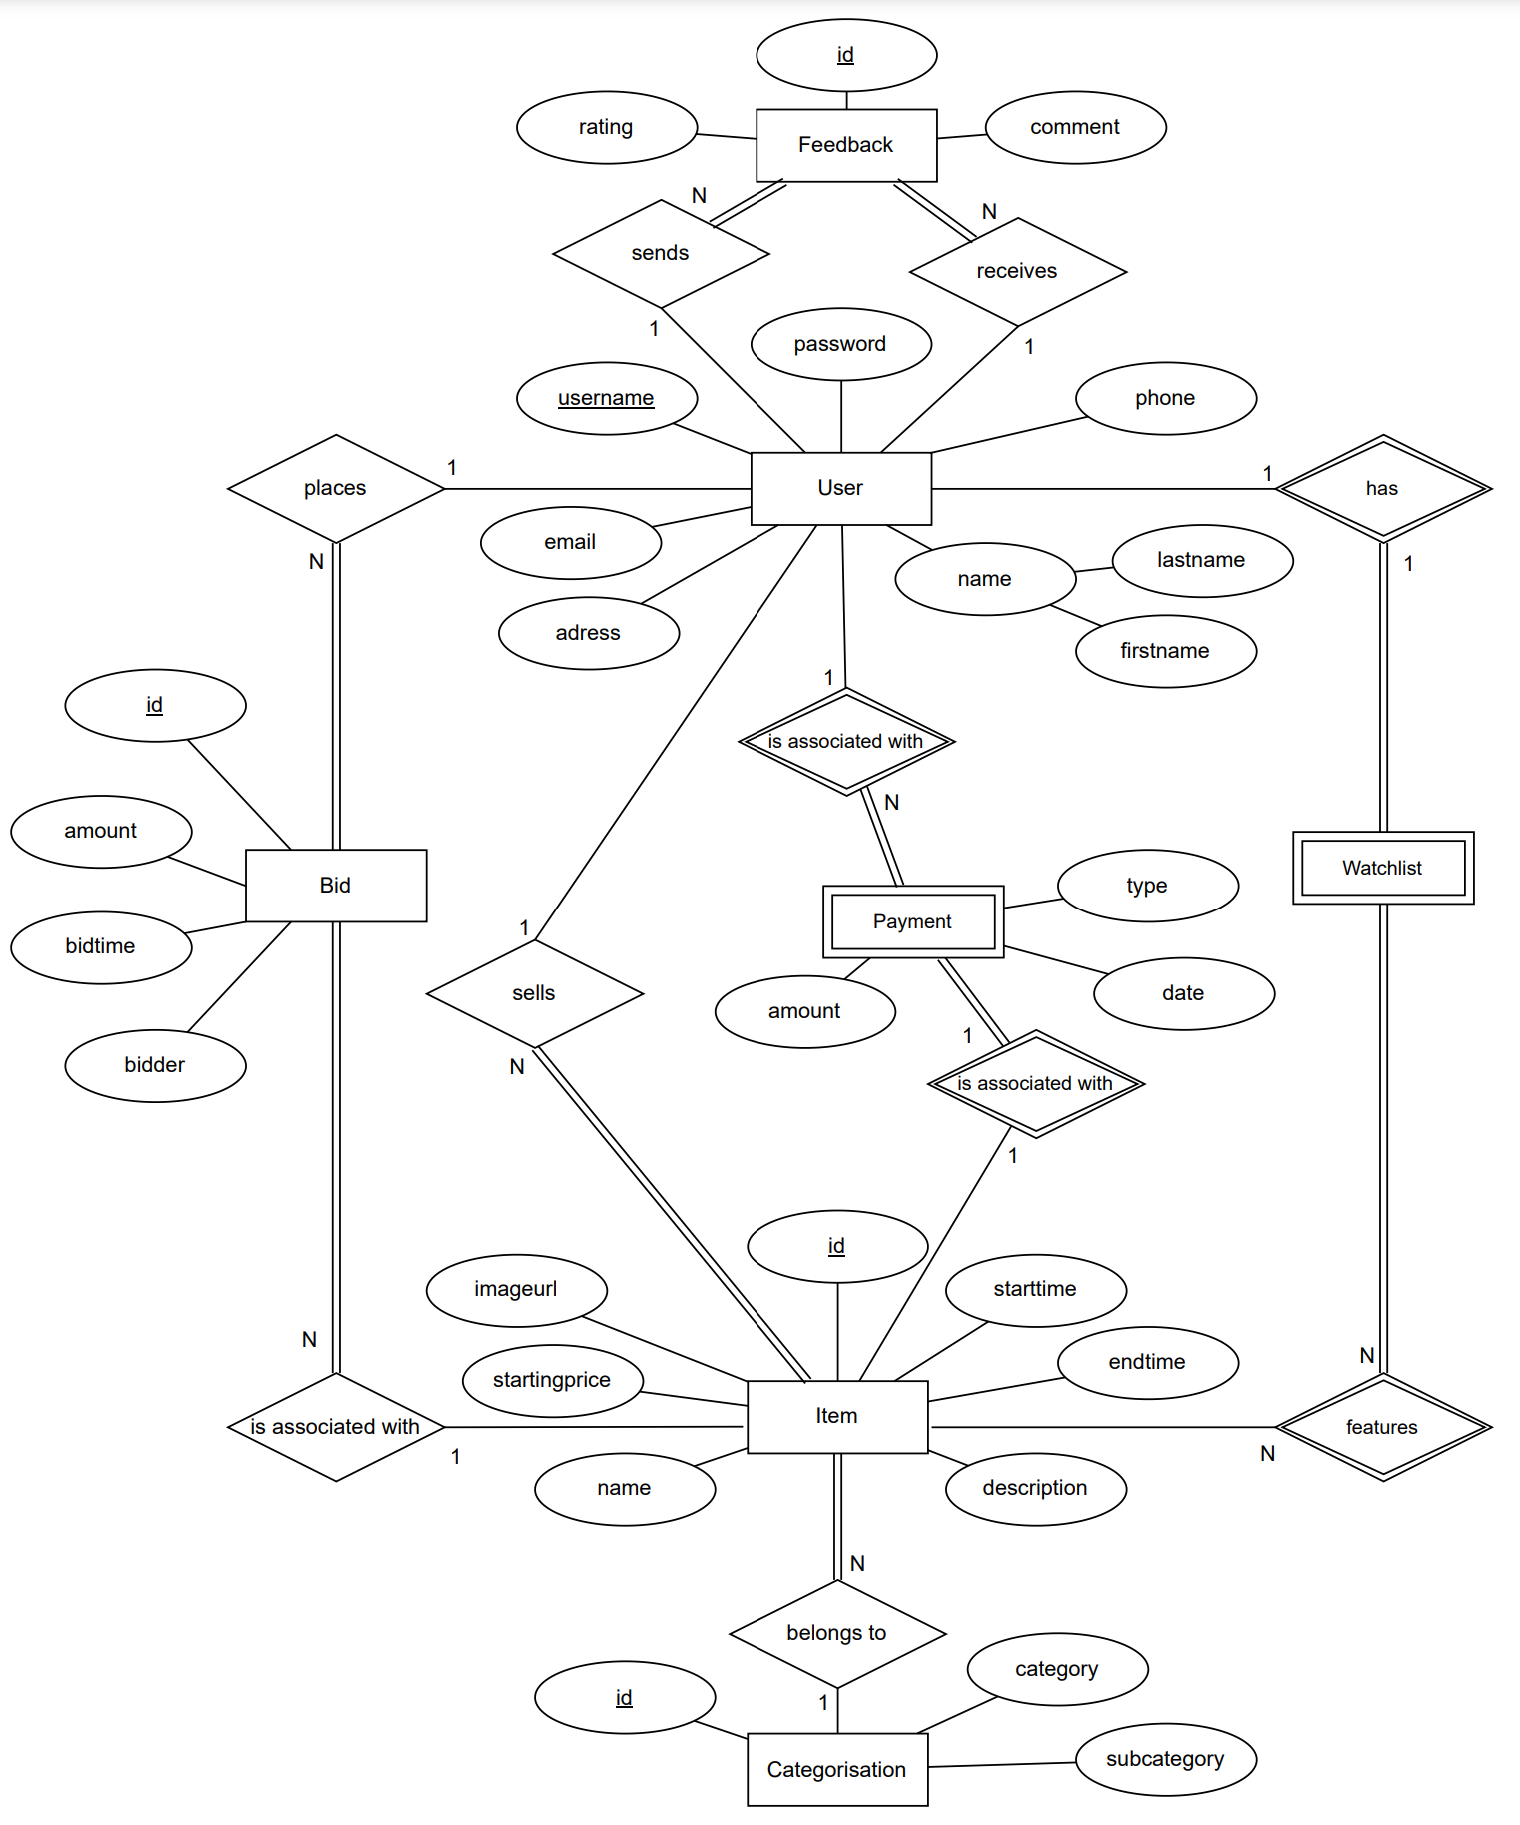
\includegraphics[height=0.65\textheight]{img/erd.png}
	\caption{Entity-Relationship Diagram}
	\label{fig:erd}
\end{figure}

\section{Tables}

The user table is designed to store all details about the users of the auction system. This includes columns such as 'username', which serves as the primary key and a unique identifier for each user, 'email', the user's unique email address, 'password', the user's hashed password for enhanced security, 'firstName' and 'lastName', which are the first and last name of the user respectively, 'name', a composite of the first and last names, 'address', the user's physical address, and 'phone', the unique phone number of the user. All attributes must have values to create a new user entry.

\begin{lstlisting}[style=sqlStyle]
	CREATE TABLE "user" (
		username VARCHAR(255) PRIMARY KEY,
		email EMAIL NOT NULL UNIQUE,
		password VARCHAR(255) NOT NULL,
		firstName VARCHAR(50) NOT NULL,
		lastName VARCHAR(50) NOT NULL,
		name VARCHAR(100) GENERATED ALWAYS AS (firstName || ' ' || lastName) STORED,
		address TEXT NOT NULL,
		phone VARCHAR(20) NOT NULL UNIQUE
	);
\end{lstlisting}

The item table is responsible for tracking all items listed for auction. It comprises columns such as 'id', a unique identifier for each item and the primary key for this table, 'name', the item's name, 'description', a detailed description of the item, 'startingPrice', the initial price for the auction of this item, 'startTime' and 'endTime', the timestamps for the beginning and end of the auction, 'imageUrl', the URL for an image of the item, 'user\_username', the username of the user who listed the item, a foreign key referencing the user table, and 'category\_id', the id of the item's category, a foreign key referencing the categorisation table.

\begin{lstlisting}[style=sqlStyle]
	CREATE TABLE Item (
		id INTEGER DEFAULT nextval('item_sequence') PRIMARY KEY,
		name VARCHAR(50) NOT NULL,
		description TEXT NOT NULL,
		startingPrice NUMERIC DEFAULT 0,
		startTime TIMESTAMP NOT NULL,
		endTime TIMESTAMP NOT NULL,
		imageUrl TEXT NOT NULL,
		user_username VARCHAR(50) REFERENCES "user"(username)
	ON DELETE SET NULL,
		category_id INTEGER REFERENCES Categorisation(id)
	);
\end{lstlisting}

The categorisation table categorizes the items being auctioned. It consists of three columns - 'id', 'category', and 'subcategory'. 'id' is a unique identifier for each category or subcategory pairing and serves as the primary key for this table. 'category' and 'subcategory' are text-based columns that describe the item category and the corresponding subcategory.

\begin{lstlisting}[style=sqlStyle]
	CREATE TABLE Categorisation (
		id SERIAL PRIMARY KEY,
		category VARCHAR(50) NOT NULL,
		subcategory VARCHAR(50) NOT NULL
	);
\end{lstlisting}

The bid table contains information regarding all bids placed on the items. It includes 'id', a unique identifier for each bid and the primary key for this table, 'amount', the bid's amount, 'bidTime', the timestamp when the bid was placed, 'user\_username', the username of the user who placed the bid, a foreign key referencing the user table, and 'item\_id', the id of the item being bid on, a foreign key referencing the item table.

\begin{lstlisting}[style=sqlStyle]
	CREATE TABLE Bid (
		id SERIAL PRIMARY KEY,
		amount NUMERIC NOT NULL,
		bidTime TIMESTAMP NOT NULL,
		user_username VARCHAR(50) REFERENCES "user"(username)
	ON DELETE SET NULL,
		item_id INTEGER REFERENCES Item(id)
	);
\end{lstlisting}

The watchlist table allows users to track items they are interested in. It includes 'user\_username', the username of the user interested in an item, a foreign key referencing the user table, and 'item\_id', the id of the item the user is interested in, a foreign key referencing the item table. The combination of 'user\_username' and 'item\_id' is unique, preventing duplicate entries in the watchlist.

\begin{lstlisting}[style=sqlStyle]
	CREATE TABLE Watchlist (
		user_username VARCHAR(50) REFERENCES "user"(username)
	ON DELETE CASCADE,
		item_id SERIAL REFERENCES Item(id),
	CONSTRAINT unique_watchlist_entry UNIQUE (user_username, item_id)
	);
\end{lstlisting}

The feedback table facilitates users in leaving feedback about their transactions. It comprises 'feedbackID', a unique identifier for each feedback and the primary key for this table, 'rating', the rating given by the sender to the receiver on a scale from 0 to 10, 'comment', a text field for additional comments, 'sender' and 'receiver', the usernames of the user giving and receiving the feedback, both foreign keys referencing the user table.

\begin{lstlisting}[style=sqlStyle]
	CREATE TABLE Feedback (
		feedbackID SERIAL PRIMARY KEY,
		rating INTEGER NOT NULL CHECK (rating BETWEEN 0 AND 10),
		comment TEXT,
		sender VARCHAR(50) REFERENCES "user"(username)
	ON DELETE SET NULL,
		receiver VARCHAR(50) REFERENCES "user"(username)
	ON DELETE SET NULL
	);
\end{lstlisting}

The payment table records all payments made for the items. It includes 'amount', the amount paid, 'date', the timestamp when the payment was made, 'type', the method of payment, 'user\_username', the username of the user making the payment, a foreign key referencing the user table, and 'item\_id', the id of the item for which the payment was made, a foreign key referencing the item table.

\begin{lstlisting}[style=sqlStyle]
	CREATE TABLE Payment (
		amount NUMERIC NOT NULL,
		date TIMESTAMP NOT NULL,
		type PAYMENT_TYPE NOT NULL,
		user_username VARCHAR(50) REFERENCES "user"(username)
	ON DELETE SET NULL,
		item_id INTEGER REFERENCES Item(id)
	);
\end{lstlisting}


\section{Relationships}
\textbf{User Table - Item Table}: Each user can list many items for auction, but each item is listed by only one user. The relationship is established via the user\_username foreign key in the Item table.

\textbf{User Table - Bid Table}: Each user can place many bids, but each bid is placed by only one user. This relationship is established via the user\_username foreign key in the Bid table.

\textbf{User Table - Watchlist Table}: Each user can have many items on their watchlist, but each watchlist entry is linked to only one user. This relationship is established via the user\_username foreign key in the Watchlist table.

\textbf{User Table - Feedback Table}: Each user can both give and receive feedback many times, but each feedback entry is given by and given to only one user. This relationship is established via the sender and receiver foreign keys in the Feedback table.

\textbf{User Table - Payment Table}: Each user can make many payments, but each payment is made by only one user. This relationship is established via the user\_username foreign key in the Payment table.

\textbf{Item Table - Bid Table}: Each item can have many bids, but each bid is placed on only one item. The relationship is established via the item\_id foreign key in the Bid table.

\textbf{Item Table - Watchlist Table}: Each item can be on the watchlist of many users, but each watchlist entry is for only one item. This relationship is established via the item\_id foreign key in the Watchlist table.

\textbf{Item Table - Payment Table}: Each item has one payment associated with it, and each payment is linked to only one item. This relationship is established via the item\_id foreign key in the Payment table.

\textbf{Categorisation Table - Item Table}: Each category can have many items, but each item belongs to only one category. The relationship is established through the category\_id foreign key in the Item table.


\section{Views}
The database also consists of two views, item\_status and user\_statistics.
The items\_status view is created to show the current status of each item in the auction. It contains various fields that provide important information about the item, its current highest bid, and the related users (highest bidder and seller). The purpose of this view is to aggregate relevant data from multiple tables and present it in a more readable and understandable format. It can be used to display the current state of items in a user-friendly way on an application or website.

The view is created by joining the item table with a subquery that calculates the highest bid for each item. The result is then joined with the bid table to retrieve the highest bidder's username. The selected fields in this view include the item's name, id, description, image URL, remaining time until the auction ends, the highest bid, the highest bidder's username, and the seller's username.
\begin{lstlisting}[style=sqlStyle]
	CREATE VIEW items_status AS
	SELECT 
		item.name AS title, 
		item.id AS item_id, 
		item.description, 
		item.imageUrl AS image_path,  
		EXTRACT(DAY FROM AGE(item.endtime, CURRENT_TIMESTAMP)) AS time_left,
		max_bids.highest_bid,
		bid.user_username AS highest_bidder,
		item.user_username AS seller
	FROM item 
	JOIN (SELECT item_id, MAX(amount) AS highest_bid FROM bid GROUP BY item_id) AS max_bids 
	ON item.id = max_bids.item_id
	JOIN bid
	ON bid.item_id = max_bids.item_id
	AND bid.amount = max_bids.highest_bid;
\end{lstlisting}

The user\_statistics materialized view in the database provides an aggregated summary of user activities on the auction platform. Being a materialized view, it stores the result of a complex and potentially time-consuming query, which can be refreshed as required, leading to faster data retrieval.

Each row in this view represents a unique user on the platform. The view contains a variety of fields calculated from different tables to give a comprehensive overview of each user's auction activities. The participated\_auctions field shows the total number of unique auctions where the user has placed a bid, as determined from the bid table. Another field, won\_auctions, displays the number of auctions that the user has won. It's calculated from the bid table, where the user's bid was the highest and the auction time had ended. The average\_rating field indicates the mean feedback rating received by the user. It's derived from the feedback table by averaging all the ratings received by a user.
To understand the financial aspect, two more fields are included: total\_expenses and total\_income. total\_expenses shows the sum of all the payments made by a user for won auctions, calculated from the payment table. On the other hand, total\_income calculates the total amount received by a user for the items they have sold. It's calculated by joining the payment and item tables and summing up the amounts where the user is the seller.

\begin{lstlisting}[style=sqlStyle]
	CREATE MATERIALIZED VIEW user_statistics AS
	SELECT 
		u.username,
		COALESCE(participated_auctions.participated_auctions, 0) AS participated_auctions,
		COALESCE(won_auctions.won_auctions, 0) AS won_auctions,
		COALESCE(CAST(average_feedback.average_rating AS INTEGER), 0) AS average_rating,
		COALESCE(total_expenses.total_expenses, 0) AS total_expenses,
		COALESCE(total_income.total_income, 0) AS total_income
	FROM "user" u
	LEFT JOIN (
	SELECT user_username, COUNT(DISTINCT item_id) AS participated_auctions
	FROM bid
	GROUP BY user_username
	) AS participated_auctions ON u.username = participated_auctions.user_username
	LEFT JOIN (
	SELECT user_username, COUNT(DISTINCT bid.item_id) AS won_auctions
	FROM bid
	JOIN items_status ON bid.item_id = items_status.item_id AND bid.amount = items_status.highest_bid
	WHERE items_status.time_left < 0
	GROUP BY user_username
	) AS won_auctions ON u.username = won_auctions.user_username
	LEFT JOIN (
	SELECT receiver, AVG(rating) AS average_rating
	FROM feedback
	GROUP BY receiver
	) AS average_feedback ON u.username = average_feedback.receiver
	LEFT JOIN (
	SELECT user_username AS buyer, SUM(amount) AS total_expenses
	FROM payment
	GROUP BY user_username
	) AS total_expenses ON u.username = total_expenses.buyer
	LEFT JOIN (
	SELECT item.user_username AS seller, SUM(amount) AS total_income
	FROM payment
	JOIN item ON item.id = payment.item_id
	GROUP BY item.user_username
	) AS total_income ON u.username = total_income.seller;
\end{lstlisting}


\section{Stored Procedure}
The purpose of the implemented stored procedure is to add a random item to the watchlist of a user when the user account is created. The item must be currently on auction, meaning its end time must be in the future.

A variable random\_item\_id of type integer is declared to store the id of a randomly selected item. It executes a SELECT query to get the id of a random item that is currently on auction. This is done by ordering the items from the items\_status view (which contains the items with their current status) randomly and selecting the first one. Once it has the id of a random item, it inserts a new row into the watchlist table with the username of the new user and the id of the randomly selected item.

This stored procedure is run by a trigger named user\_created\_trigger. A trigger is a special type of stored procedure that runs automatically when an event associated with a table occurs such as insert, update, or delete. In this case, the trigger is configured to run the add\_random\_item\_to\_watchlist() stored procedure each time a new row is inserted into the user table. This is specified by the AFTER INSERT ON "user" part of the trigger creation statement.

\begin{lstlisting}[style=sqlStyle]
	CREATE OR REPLACE FUNCTION add_random_item_to_watchlist()
	RETURNS TRIGGER AS $$
	DECLARE
		random_item_id INTEGER;
	BEGIN
	
	-- Get the id of a random item which is currently on auction
	SELECT item_id
	FROM items_status
	WHERE time_left > 0
	ORDER BY RANDOM()
	LIMIT 1
	INTO random_item_id;
	
	-- Put that item on the watchlist of the newly created user
	INSERT INTO watchlist (user_username, item_id)
	VALUES (NEW.username, random_item_id);
	
	RETURN NEW;
	END;
	
	$$ LANGUAGE plpgsql;
	
	-- Create a trigger that executes the stored procedure whenever a new entry is added to the user table
	CREATE TRIGGER user_created_trigger
	AFTER INSERT ON "user"
	FOR EACH ROW
	EXECUTE FUNCTION add_random_item_to_watchlist();
\end{lstlisting}

% !TEX root =  master.tex
\chapter{Normalization Analysis}
Normalization is a database design technique that reduces data redundancy and eliminates undesirable characteristics like Insertion, Update and Deletion Anomalies. Normal forms are a set of conditions or rules that a relation (table) in a database must adhere to, to qualify as a 'good' structure. This analysis will check whether the relations in the database meet at least the Third Normal Form (3NF).


\begin{table}[h]
	\centering
	\begin{tabular}{|c|p{10cm}|}
		\hline
		\textbf{Normal Form} & \textbf{Definition} \\
		\hline
		First Normal Form (1NF) & A relation is in 1NF if it contains an atomic value for each attribute (column) in a record (row). It should also have a primary key that uniquely identifies each record. \\
		\hline
		Second Normal Form (2NF) & A relation is in 2NF if it is in 1NF and all non-key attributes are fully functionally dependent on the primary key. This essentially means there is no partial dependency of any column on the primary key. \\
		\hline
		Third Normal Form (3NF) & A relation is in 3NF if it is in 2NF and no non-key attribute is transitively dependent on the primary key. \\
		\hline
	\end{tabular}
	\caption{Definitions of Normal Forms}
	\label{tab:normal_forms}
\end{table}



\textbf{1. Categorisation Table}
The Categorisation table consists of three attributes: id, category, and subcategory. The primary key is 'id', and every 'id' refers to a unique category and subcategory. There are no duplicate or redundant data, and every attribute is atomic, which satisfies 1NF.
Since there's only one candidate key (id), and all non-key attributes (category and subcategory) are fully dependent on it, 2NF is satisfied.
There's no transitive dependency as there's only one candidate key, and thus the table also satisfies 3NF.


\textbf{2. User Table}
The 'user' table has eight attributes: username, email, password, firstName, lastName, name, address, and phone. The primary key is 'username', and every 'username' refers to a unique user record.
However, the 'name' attribute is a derived attribute (it's generated always as the concatenation of 'firstName' and 'lastName'). This breaks the rule of 1NF as it introduces redundancy. To satisfy 1NF, we could remove the 'name' attribute and derive it in our queries when needed.
Assuming we consider the 'name' attribute as not violating 1NF, the table would meet the conditions for 2NF as there's only one candidate key, and all non-key attributes are fully dependent on it.
For 3NF, the table doesn't have any non-key attribute that is transitively dependent on the primary key, so it satisfies 3NF as well.


\textbf{3. Item Table}
The Item table has nine attributes: id, name, description, startingPrice, startTime, endTime, imageUrl, user\_username, and category\_id. The primary key is 'id', and every 'id' refers to a unique item.
The table is in 1NF as all attributes are atomic, and each record is unique.
The table is in 2NF as all non-key attributes are fully dependent on the primary key.
The table is in 3NF as there are no transitive dependencies.


\textbf{4. Bid Table}
The Bid table is in 1NF, 2NF, and 3NF. All attributes are atomic, each record is uniquely identified by 'id', all non-key attributes are fully dependent on the primary key, and there are no transitive dependencies.


\textbf{5. Watchlist Table}
The Watchlist table has two attributes: user\_username and item\_id. The primary key is a combination of 'user\_username' and 'item\_id', and every combination refers to a unique watchlist entry.
The table is in 1NF as all attributes are atomic, and each record is unique.
The table is in 2NF as there are no non-key attributes, so the condition of full functional dependency is trivially satisfied.
The table is also in 3NF as there are no transitive dependencies.


All tables in the given SQL code are in the Third Normal Form (3NF), assuming that the 'name' attribute in the 'user' table doesn't violate the 1NF. If it does, the 'user' table should be modified by removing the 'name' attribute to meet 1NF, 2NF, and 3NF.
% !TEX root =  master.tex

\chapter{SQL Queries and Indices}
The fields 'item\_id' and 'amount' where indexed in order to significantly improve the performance of queries that involve filtering, searching, or joining based on these columns. 

\begin{lstlisting}[style=sqlStyle]
	CREATE INDEX index_bid_item_id ON Bid (item_id);
	CREATE INDEX index_bid_amount ON Bid (amount);
\end{lstlisting}

This increases efficiency considerably since those columns used to create the database view 'items\_status', which in turn is accessed in 5 separate queries, including those that are the used most frequently. In total our web application uses 22 separate queries which were implemented using psycopg2, 7 of which will be explained in this chapter.

\begin{lstlisting}[style=sqlStyle]
SELECT 
	items_status.*,
	CASE
		WHEN filtered_watchlist.user_username is NUll THEN 0
		ELSE 1
	END as is_watchlist
FROM items_status 
	LEFT JOIN (
		SELECT * FROM watchlist WHERE user_username = '{self.__current_user}'
	) AS filtered_watchlist ON items_status.item_id = filtered_watchlist.item_id 
WHERE items_status.time_left > 0;
\end{lstlisting}

This nested query retrieves active items from the items\_status view and adds an additional column that indicates whether the item is in the users watchlist or not.

\begin{lstlisting}[style=sqlStyle]
	REFRESH MATERIALIZED VIEW user_statistics;
	SELECT * FROM user_statistics WHERE username = '{self.__current_user}';
\end{lstlisting}
This query refreshes the materialized view user\_statistics and retrieves statistics data such as the number of won auctions or the total income generated via sold items for the current user.

\begin{lstlisting}[style=sqlStyle]
SELECT DISTINCT
	items_status.item_id, 
	title, 
	description, 
	image_path, 
	highest_bid AS amount, 
	CASE 
		WHEN highest_bidder = '{self.__current_user}' THEN 'buyer'
		WHEN seller = '{self.__current_user}' THEN 'seller'
	END AS role,
	CASE 
		WHEN feedback.rating IS NULL THEN 0
		ELSE 1
	END AS has_feedback
FROM items_status 
	LEFT JOIN feedback ON items_status.item_id = feedback.item_id
WHERE time_left <= 0 AND (highest_bidder = '{self.__current_user}' OR seller = '{self.__current_user}');
\end{lstlisting}
This query retrieves the completed auctions in which the current user participated either as a buyer or a seller. It includes information such as item ID, title, description, image path, highest bid amount and the user's role. The field 'has\_feedback' contains the information wether the user already send feedback to the other user which won or sold the item. The frontend uses this information to either display or hide the possibility to give feedback.

\begin{lstlisting}[style=sqlStyle]
UPDATE \"user\" SET {filled_inputs} WHERE username = '{self.__current_user}';
\end{lstlisting}
This query updates the user's personal data in the user table. It takes the email, first name, last name, address, and phone as input values and updates the corresponding columns for the current user.

\begin{lstlisting}[style=sqlStyle]
DELETE FROM watchlist WHERE user_username = '{self.__current_user}' AND item_id = '{item_id}'
\end{lstlisting}
This query deletes the user's data from the user table. Other tables which reference the user table utilize 'ON DELETE SET NULL'. This way the statistics and auction histories of other users are not impaired once a user is deleted.

\begin{lstlisting}[style=sqlStyle]
SELECT 
	highest_bid AS amount, 
	item.endtime AS date,
	CASE FLOOR(RANDOM() * 3)
		WHEN 0 THEN 'Cash'
		WHEN 1 THEN 'Credit Card'
		WHEN 2 THEN 'Paypal'
	END AS type,	
	items_status.highest_bidder AS user_username,
	items_status.item_id
FROM items_status
	LEFT JOIN payment ON items_status.item_id = payment.item_id
	JOIN item ON items_status.item_id = item.id
WHERE time_left <= 0 AND payment.amount IS NULL AND highest_bid > 0;

INSERT INTO payment VALUES ({auction["amount"]}, '{auction["date"]}', '{auction["type"]}', '{auction["user_username"]}', {auction["item_id"]});
\end{lstlisting}
This query retrieves information about auctions that have ended but do not have a corresponding payment yet. It then chooses a payment type at random and inserts a corresponding entry in the 'payment' table. It was implemented for demonstration purposes and simulates a direct debit collection for an item whose auction has endet. Because the scope of this university project does not allow hosting a server which automatically executes this query at the very second that the auction has endet, we had to come up with a different solution. That's why this query is triggered each time any other query is executed. This way it is ensured that the user immediately sees updated informations (e.g. user statistics or payment info) once an auction has endet and he interacted with the website. Again this is just for demonstration purposes and we are well aware that this would not be a feasable solution in a real world scenario.


%% !TEX root =  master.tex

\chapter{Application}



% Fazit und Ausblick
%% !TEX root =  master.tex
\chapter{Zusammenfassung}

\nocite{*}

Dieses Kapitel enthält die Zusammenfassung der Arbeit mit Fazit und Ausblick.

\section{Fazit}

...

\section{Ausblick}

...


%%%%%%%%%%%%%%%%%%%%%%%%%%%%%%%%%%%

%%%%%%%%%%%%%%%%%%%%%%%%%%%%%%%%%%%
% ANHÄNGE
%
% @stud: einzelne Anhänge bearbeiten und eigene Anhänge hier einfügen 
%        die nachfolgenden Zeilen deaktivieren, wenn keine Anhänge verwendet werden
%
%\initializeAppendix
%% !TEX root =  master.tex
\chapter{Beispiel-Anhang: Testanhang}

%% !TEX root =  master.tex
\chapter{Beispiel-Anhang: Noch ein Testanhang}
nochmal: lipsum ...

%%%%%%%%%%%%%%%%%%%%%%%%%%%%%%%%%%%

\singlespacing

%%%%%%%%%%%%%%%%%%%%%%%%%%%%%%%%%%%
% LITERATURVERZEICHNIS
% @stud: Literaturverzeichnis in Datei bibliography.bib anpassen. 
%
% Alternative zu Verwendung von \initializeBibliography: Citavi ...
% (dann \initializeBibliography auskommentieren und eigenes LaTex Coding verwenden)
%
\initializeBibliography
%%%%%%%%%%%%%%%%%%%%%%%%%%%%%%%%%%%

%%%%%%%%%%%%%%%%%%%%%%%%%%%%%%%%%%%
% INDEX
% @stud: ggf. Index auskommentieren, wenn nicht benötigt
%
\addcontentsline{toc}{chapter}{Index}
\printindex

\end{document}
